% This file was created by tikzplotlib vunknown.
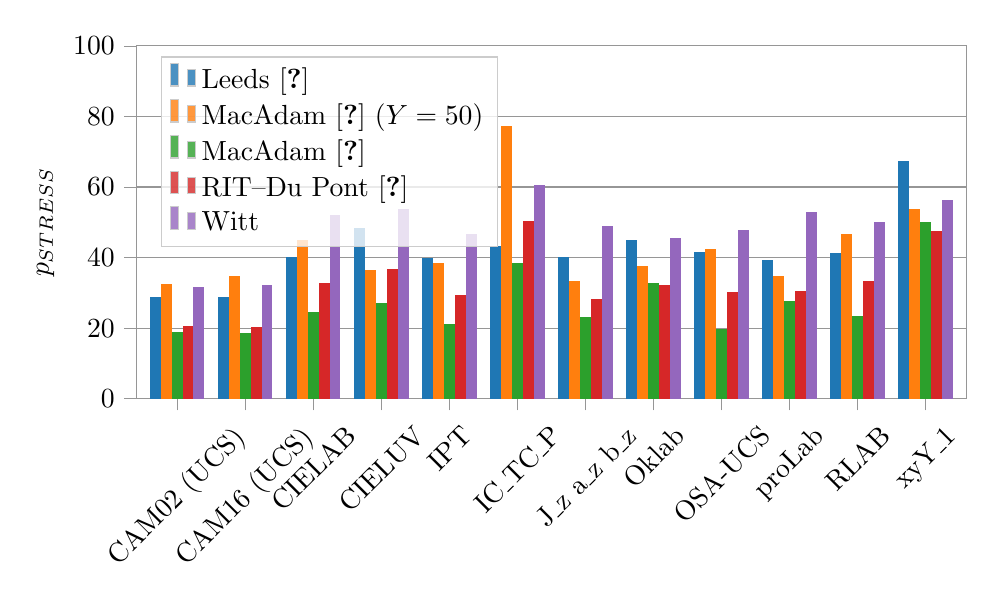
\begin{tikzpicture}

\definecolor{color0}{rgb}{0.12156862745098,0.466666666666667,0.705882352941177}
\definecolor{color1}{rgb}{1,0.498039215686275,0.0549019607843137}
\definecolor{color2}{rgb}{0.172549019607843,0.627450980392157,0.172549019607843}
\definecolor{color3}{rgb}{0.83921568627451,0.152941176470588,0.156862745098039}
\definecolor{color4}{rgb}{0.580392156862745,0.403921568627451,0.741176470588235}

\begin{axis}[
axis line style={white!58.8235294117647!black},
height=0.5\textwidth,
legend cell align={left},
legend style={fill opacity=0.8, draw opacity=1, text opacity=1, at={(0.03,0.97)}, anchor=north west, draw=white!80!black},
tick align=outside,
tick pos=left,
width=\textwidth,
x grid style={white!58.8235294117647!black},
xmin=-0.6, xmax=11.6,
xtick style={color=white!58.8235294117647!black},
xtick={0,1,2,3,4,5,6,7,8,9,10,11},
xticklabel style = {rotate=45.0},
xticklabels={CAM02 (UCS),CAM16 (UCS),CIELAB,CIELUV,IPT,IC\_TC\_P,J\_z a\_z b\_z,Oklab,OSA-UCS,proLab,RLAB,xyY\_1},
y grid style={white!58.8235294117647!black},
ylabel={\(\displaystyle p_{STRESS}\)},
ymajorgrids,
ymin=0, ymax=100,
ytick style={color=white!58.8235294117647!black}
]
\draw[draw=none,fill=color0] (axis cs:-0.4,0) rectangle (axis cs:-0.24,28.6919923366331);
\addlegendimage{ybar,ybar legend,draw=none,fill=color0};
\addlegendentry{Leeds \cite{leeds}}

\draw[draw=none,fill=color0] (axis cs:0.6,0) rectangle (axis cs:0.76,28.7161180400034);
\draw[draw=none,fill=color0] (axis cs:1.6,0) rectangle (axis cs:1.76,40.0364176602205);
\draw[draw=none,fill=color0] (axis cs:2.6,0) rectangle (axis cs:2.76,48.2883322241465);
\draw[draw=none,fill=color0] (axis cs:3.6,0) rectangle (axis cs:3.76,39.8577462530719);
\draw[draw=none,fill=color0] (axis cs:4.6,0) rectangle (axis cs:4.76,43.163489790704);
\draw[draw=none,fill=color0] (axis cs:5.6,0) rectangle (axis cs:5.76,40.1250346751512);
\draw[draw=none,fill=color0] (axis cs:6.6,0) rectangle (axis cs:6.76,45.0479667569395);
\draw[draw=none,fill=color0] (axis cs:7.6,0) rectangle (axis cs:7.76,41.6629221789247);
\draw[draw=none,fill=color0] (axis cs:8.6,0) rectangle (axis cs:8.76,39.1911679982171);
\draw[draw=none,fill=color0] (axis cs:9.6,0) rectangle (axis cs:9.76,41.337101933465);
\draw[draw=none,fill=color0] (axis cs:10.6,0) rectangle (axis cs:10.76,67.2537962599619);
\draw[draw=none,fill=color1] (axis cs:-0.24,0) rectangle (axis cs:-0.08,32.4164992368733);
\addlegendimage{ybar,ybar legend,draw=none,fill=color1};
\addlegendentry{MacAdam \cite{macadam1942} ($Y=50$)}

\draw[draw=none,fill=color1] (axis cs:0.76,0) rectangle (axis cs:0.92,34.7611229410046);
\draw[draw=none,fill=color1] (axis cs:1.76,0) rectangle (axis cs:1.92,44.8952155515788);
\draw[draw=none,fill=color1] (axis cs:2.76,0) rectangle (axis cs:2.92,36.5010276032748);
\draw[draw=none,fill=color1] (axis cs:3.76,0) rectangle (axis cs:3.92,38.4833636095126);
\draw[draw=none,fill=color1] (axis cs:4.76,0) rectangle (axis cs:4.92,77.2316903365112);
\draw[draw=none,fill=color1] (axis cs:5.76,0) rectangle (axis cs:5.92,33.2757088119242);
\draw[draw=none,fill=color1] (axis cs:6.76,0) rectangle (axis cs:6.92,37.6772548200669);
\draw[draw=none,fill=color1] (axis cs:7.76,0) rectangle (axis cs:7.92,42.4396646797378);
\draw[draw=none,fill=color1] (axis cs:8.76,0) rectangle (axis cs:8.92,34.635501753967);
\draw[draw=none,fill=color1] (axis cs:9.76,0) rectangle (axis cs:9.92,46.581942046651);
\draw[draw=none,fill=color1] (axis cs:10.76,0) rectangle (axis cs:10.92,53.7506022511023);
\draw[draw=none,fill=color2] (axis cs:-0.08,0) rectangle (axis cs:0.08,19.0009867390654);
\addlegendimage{ybar,ybar legend,draw=none,fill=color2};
\addlegendentry{MacAdam \cite{macadam1974}}

\draw[draw=none,fill=color2] (axis cs:0.92,0) rectangle (axis cs:1.08,18.7044908430827);
\draw[draw=none,fill=color2] (axis cs:1.92,0) rectangle (axis cs:2.08,24.5319191673876);
\draw[draw=none,fill=color2] (axis cs:2.92,0) rectangle (axis cs:3.08,27.1465135470917);
\draw[draw=none,fill=color2] (axis cs:3.92,0) rectangle (axis cs:4.08,21.2696481498459);
\draw[draw=none,fill=color2] (axis cs:4.92,0) rectangle (axis cs:5.08,38.4505318024105);
\draw[draw=none,fill=color2] (axis cs:5.92,0) rectangle (axis cs:6.08,23.2111338532765);
\draw[draw=none,fill=color2] (axis cs:6.92,0) rectangle (axis cs:7.08,32.7178547285273);
\draw[draw=none,fill=color2] (axis cs:7.92,0) rectangle (axis cs:8.08,19.8475379525657);
\draw[draw=none,fill=color2] (axis cs:8.92,0) rectangle (axis cs:9.08,27.7092844635432);
\draw[draw=none,fill=color2] (axis cs:9.92,0) rectangle (axis cs:10.08,23.5028573394472);
\draw[draw=none,fill=color2] (axis cs:10.92,0) rectangle (axis cs:11.08,50.0184864244504);
\draw[draw=none,fill=color3] (axis cs:0.08,0) rectangle (axis cs:0.24,20.4545132821738);
\addlegendimage{ybar,ybar legend,draw=none,fill=color3};
\addlegendentry{RIT--Du Pont \cite{berns}}

\draw[draw=none,fill=color3] (axis cs:1.08,0) rectangle (axis cs:1.24,20.2056013977758);
\draw[draw=none,fill=color3] (axis cs:2.08,0) rectangle (axis cs:2.24,32.8516243171421);
\draw[draw=none,fill=color3] (axis cs:3.08,0) rectangle (axis cs:3.24,36.8498052149805);
\draw[draw=none,fill=color3] (axis cs:4.08,0) rectangle (axis cs:4.24,29.2367169724054);
\draw[draw=none,fill=color3] (axis cs:5.08,0) rectangle (axis cs:5.24,50.293188154606);
\draw[draw=none,fill=color3] (axis cs:6.08,0) rectangle (axis cs:6.24,28.3631310307662);
\draw[draw=none,fill=color3] (axis cs:7.08,0) rectangle (axis cs:7.24,32.1818564157314);
\draw[draw=none,fill=color3] (axis cs:8.08,0) rectangle (axis cs:8.24,30.1557845243711);
\draw[draw=none,fill=color3] (axis cs:9.08,0) rectangle (axis cs:9.24,30.4088657542895);
\draw[draw=none,fill=color3] (axis cs:10.08,0) rectangle (axis cs:10.24,33.2993029128068);
\draw[draw=none,fill=color3] (axis cs:11.08,0) rectangle (axis cs:11.24,47.6010340040916);
\draw[draw=none,fill=color4] (axis cs:0.24,0) rectangle (axis cs:0.4,31.7137459831053);
\addlegendimage{ybar,ybar legend,draw=none,fill=color4};
\addlegendentry{Witt}

\draw[draw=none,fill=color4] (axis cs:1.24,0) rectangle (axis cs:1.4,32.2820907703781);
\draw[draw=none,fill=color4] (axis cs:2.24,0) rectangle (axis cs:2.4,52.0435566262912);
\draw[draw=none,fill=color4] (axis cs:3.24,0) rectangle (axis cs:3.4,53.6345292231793);
\draw[draw=none,fill=color4] (axis cs:4.24,0) rectangle (axis cs:4.4,46.7942036538384);
\draw[draw=none,fill=color4] (axis cs:5.24,0) rectangle (axis cs:5.4,60.5745704771068);
\draw[draw=none,fill=color4] (axis cs:6.24,0) rectangle (axis cs:6.4,48.9109932127749);
\draw[draw=none,fill=color4] (axis cs:7.24,0) rectangle (axis cs:7.4,45.5094725773093);
\draw[draw=none,fill=color4] (axis cs:8.24,0) rectangle (axis cs:8.4,47.7458622476438);
\draw[draw=none,fill=color4] (axis cs:9.24,0) rectangle (axis cs:9.4,52.9076713909836);
\draw[draw=none,fill=color4] (axis cs:10.24,0) rectangle (axis cs:10.4,50.153271892121);
\draw[draw=none,fill=color4] (axis cs:11.24,0) rectangle (axis cs:11.4,56.1700478114188);
\end{axis}

\end{tikzpicture}
